

\chapter{Results}



\section{Fully balanced model}

The objective of this research is to understand the effects of adversarial attacks on imbalanced CNNs. However, it is firstly required to create the baseline for our comparisons. This consists of creating perturbation on every class label and querying its accuracy on a fully balanced model. Canonical models assume that every object in the dataset are sampled from similar distributions. However, in real-life situations, even though the number of samples is the same, some class labels could be poorly represented by the lack of a clear structure. This could often lead to differences in the output for each specific class \cite{krawczyk2016learning}. On this way, a superficially balanced dataset does not guarantee that the model will equally generalise across all classes.
\begin{figure}[H]
	\centering
	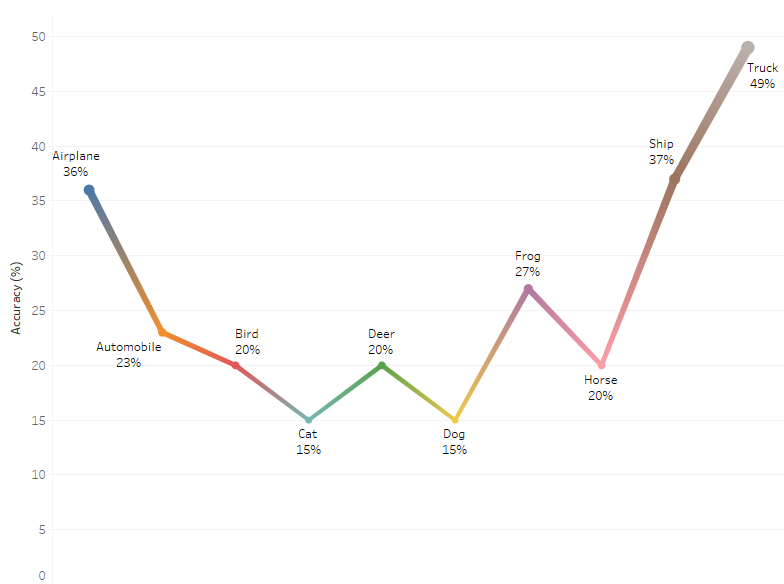
\includegraphics[scale=0.7]{balanced_perturbed.png}
	\caption{Individual class perturbed accuracy on the balanced model}
	\label{fig:balanced_perturbed}
\end{figure}

Figure ~\ref{fig:balanced_perturbed} shows that the accuracy for all classes is drastically reduced when the balanced model is presented with adversarial examples. Even though there is enough samples for each class, the adversarial attack forces the domain shift of each individual sample towards different regions in space, causing a misclassification of the current label. The effectiveness of the adversarial attack can be partially explained by the balancing of the dataset itself. In a model where the dataset used in training aims for normalization over all classes, the network is often caught in trying to find weights and biases that generalizes well over all set of labels. Therefore, perturbations become more efficient due to a bigger proximity of classes distributions in space.


\section{Class undersampling and oversampling}

The adversarial test shows the results from two perspectives. First, on the class under-sampling with same model the accuracy for each individual class was on average 15\%, which already demonstrates higher vulnerability when compared to the balanced case. This could be explained by having the data distribution of that specific class being squished into a smaller space and, hence, decreasing the amount of perturbation required to effectively increase the cost function so as to a misclassification to happen. Therefore, the degree of the perturbation required is reduced since the class label did not explore the feature space accordingly. Second, when oversampling occurs, it is expected to have the target class expanding into space and taking as much space as possible when compared to other classes. This happens since the network performs more gradient updates on that specific class due to the amount of available samples. Perturbation on this case had a lower effect, as the small push cause by our $\epsilon$ was not enough to move points to outside of their distributions.



\begin{table}[H]
	\centering
	
	\begin{tabular}{lccccc}
		\toprule
		&\multicolumn{2}{c}{Different Model}
		&\multicolumn{3}{c}{Same Model}
		\\\cmidrule(r){2-3}\cmidrule(l){4-6}
		Class Label &Undersample &Oversample &Balanced &Undersample &Oversample \\
		\midrule
		0 - Airplane &60\%& 87\% &36\%& 19\%    & 61\% \\
		1 - Automobile &64\%& 91\% &23\%& 16\%    & 63\% \\
		2 - Bird &38\%& 73\% &20\%& 9.4\%    & 27\% \\
		3 - Cat &21\%& 72\% &11\%& 0.5\%    & 19\% \\
		4 - Deer &58\%& 80\% &20\%& 9.8\%    & 20\% \\
		5 - Dog &47\%& 76\% &15\%& 9\%    & 38\% \\
		6 - Frog &76\%& 88\% &27\%& 20\%    & 49\% \\
		7 - Horse &59\%& 88\% &20\%& 18\%    & 52\% \\
		8 - Ship &69\%& 89\% &37\%& 19\%    & 59\% \\
		9 - Truck &46\%& 87\% &49\%& 21\%    & 54\% \\
		\bottomrule
	\end{tabular}
	\caption{Results for the two different sources of perturbations along with the two different imbalanced datasets}
	\label{tbl:results}
\end{table}

As the number of samples on a target class goes down, an increase of vulnerability towards that specific label is expected when compared to the balanced model. The results on table  ~\ref{tbl:results} confirms this. Networks with imbalanced datasets were more vulnerable when presented with adversarial examples. Figure ~\ref{fig:relative_difference} shows the relative difference for all the three networks (balanced, under-sampled and oversampled).  The values were calculated by finding the ratio between the new accuracy and the non-perturbed accuracy. They represent the percentage on which the initial accuracy was reduced. The under-sampled model had the higher relative difference on average, which shows that the imbalanced nature of the dataset ended-up increasing the vulnerability of the model. This poses threats to current systems as the low amount of samples during training for a specific class would  create gaps that are more easily exploited when compared to a balanced network.

\begin{figure}[H]
	\centering
	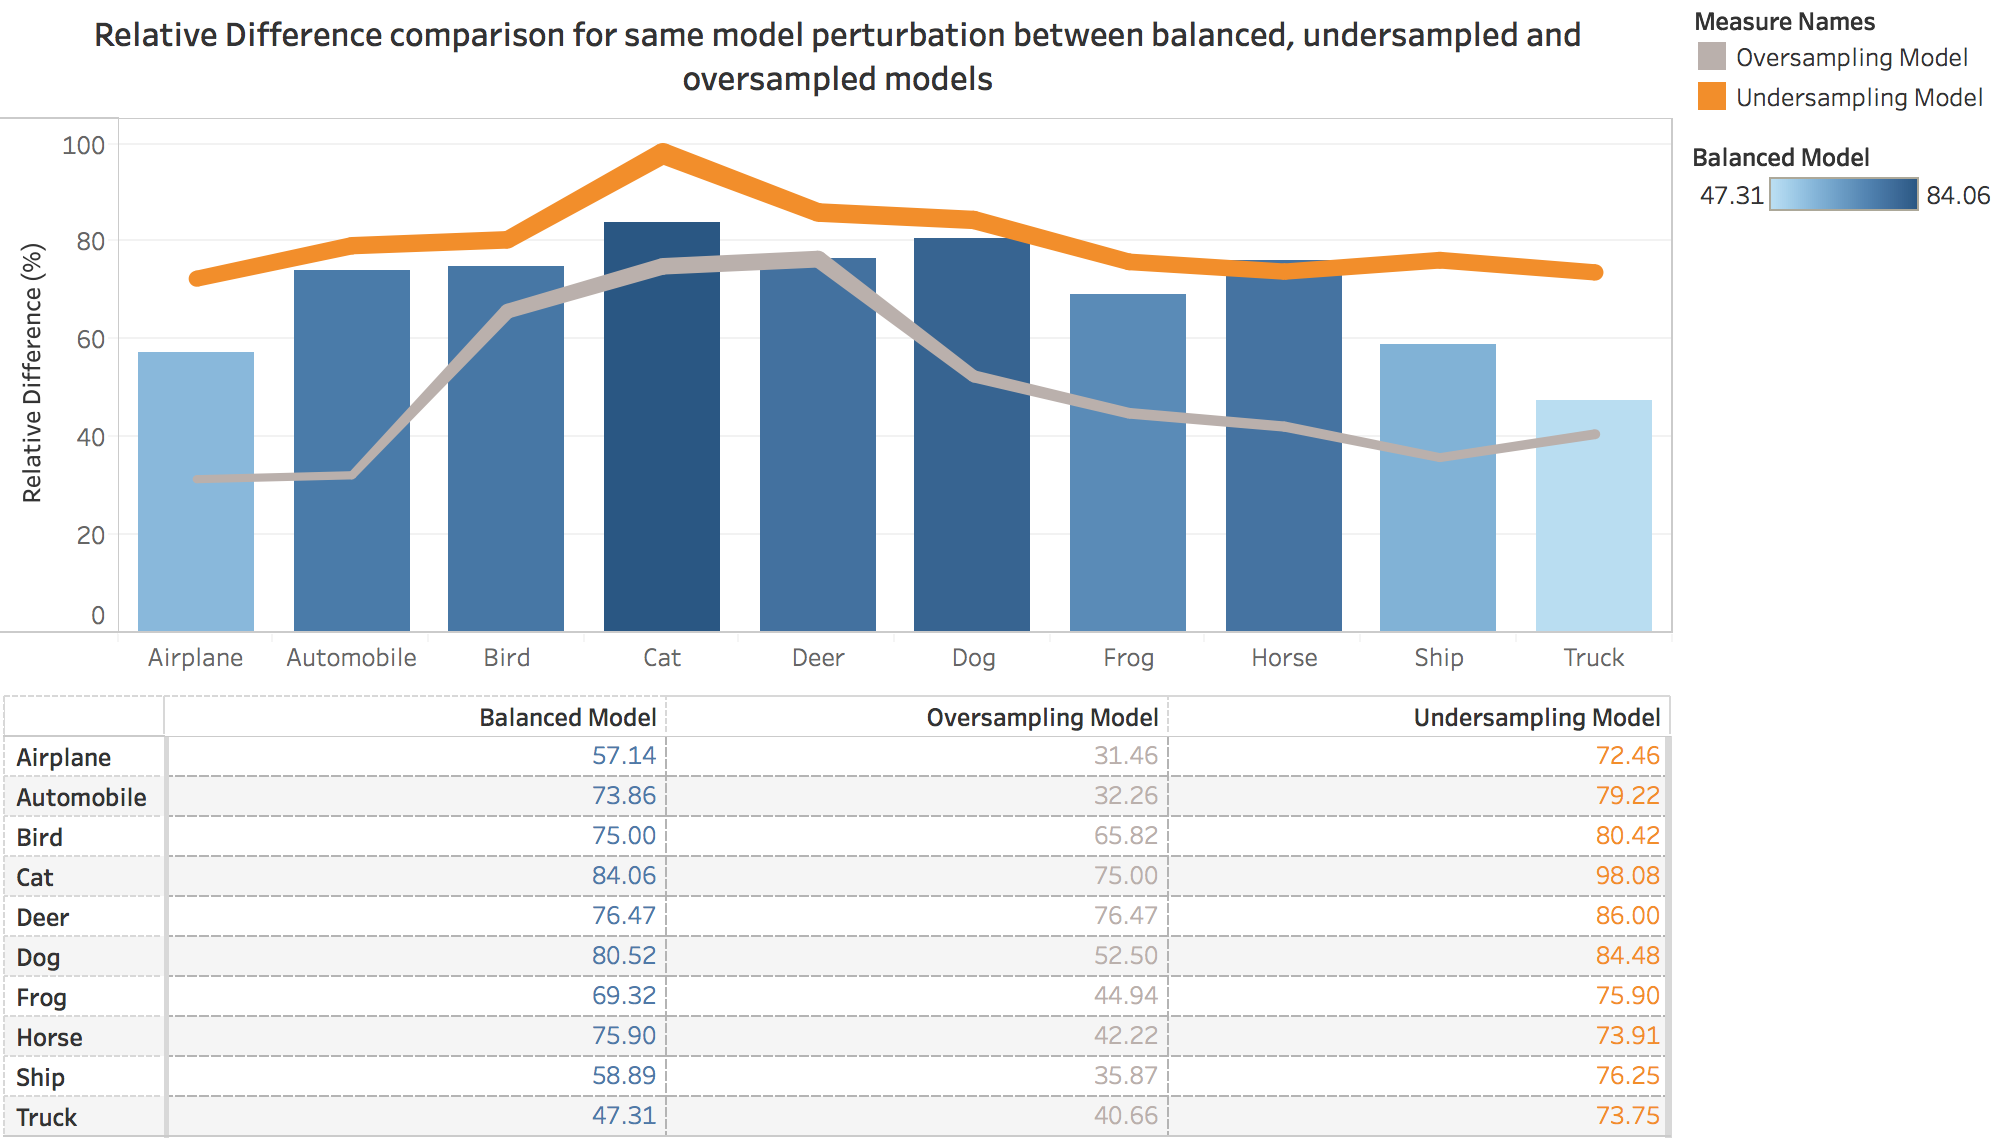
\includegraphics[scale=0.3]{rel_diff_graph.png}
	\caption{Relative difference for each model. Higher numbers means more vulnerability}
	\label{fig:relative_difference}
\end{figure}

\section{Transfer Learning}

Chapter 4 discussed different ways in which one algorithm could learn from existing models. When the attacker has no knowledge of the underlying model that he/she wants to attack, the best way to learn the gradient information is by querying the target and training a new model with its outputs. The use of a different model for creating adversaries has shown less effective when compared to the same model attack. As the overall gradient have not only different direction but also magnitudes, the attacked system has proven to be more robust. The experiment reveals that although Gradient Sign is quite effective for fooling networks it does require a good amount of knowledge from the underlying training parameters so as to unleash its full potential.

\section{Overlapping distributions}
When objects in the dataset already have distributions that are very close to one another the effects of adversarial seems to be stronger. Figure ~\ref{fig:conf_matrix_full} shows that for the pairs Cat/Dog and Automobile/Truck, misclassification naturally happens towards one another due to similarities in their feature space \cite{stanford2016}. On this case, our experiment shows that the adversarial attack intensifies the property by increasing the number on which one class is picked over another. This property gives interesting insights, as it shows that the gradient sign is really navigating around the target class distribution and when a overlap occurs it becomes easier to create an adversarial.

\begin{figure}[ht] 
	\label{fig7} 
	\begin{minipage}[b]{0.5\linewidth}
		\centering
		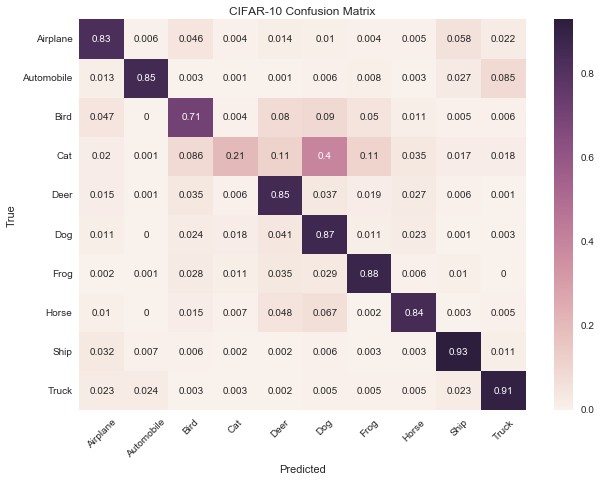
\includegraphics[width=1\linewidth]{cat_undersampling_per.png} 
		\vspace{4ex}
	\end{minipage}%%
	\begin{minipage}[b]{0.5\linewidth}
		\centering
		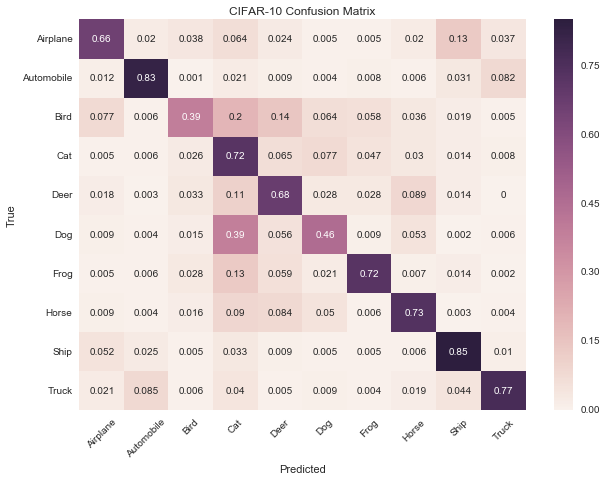
\includegraphics[width=1\linewidth]{cat_oversampling_per.png} 
		\vspace{4ex}
	\end{minipage} 
	\begin{minipage}[b]{0.5\linewidth}
		\centering
		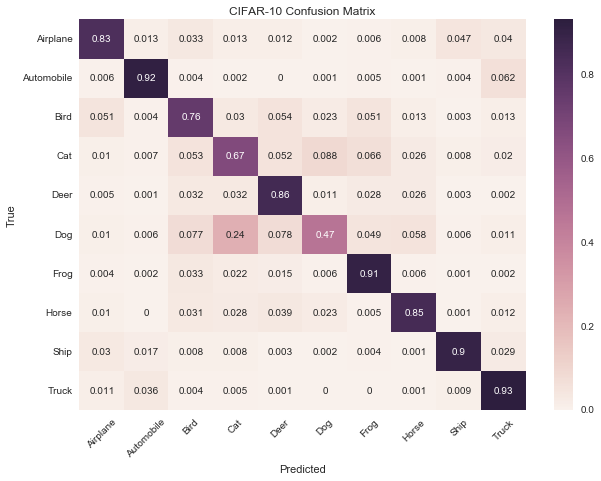
\includegraphics[width=1\linewidth]{dog_undersampling_per.png} 
		\vspace{4ex}
	\end{minipage}%% 
	\begin{minipage}[b]{0.5\linewidth}
		\centering
		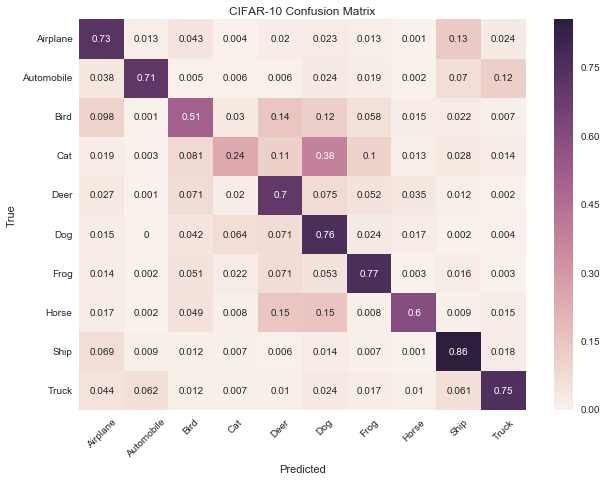
\includegraphics[width=1\linewidth]{dog_oversampling_per.png} 
		\vspace{4ex}
	\end{minipage} 
	\centering
	\caption{Top Left and Right: Cat undersampling / oversampling with perturbation. Bottom Left and Right: Dog undersampling / oversampling with perturbation}
\end{figure}

Classes with overlapping distributions sheds some light on the effect of the $\epsilon$ value of the gradient sign method. Its clear to understand that classes that are close together in the data space are required to take smaller steps in order to be successfully miss-classified. Both dog and cat classes were already being confused with one another before the adversarial attack, and the small "push" of the Gradient method has increased this effect, showing that domain shift is even stronger on these situations. The required amount of steps for classes with high level of uncertainty around them is often smaller when compared to classes with a better and more confident exploration of space.